\chapter{Attack simulation}
\label{cap:attacksimulations}

% ES-CMA reliability based

\section{Detection of unstable challenges}
% mv vs. measurements
% unstable challenges are required for the cma-es attack
% Finding unstable challenges: graph!
%========================================

\begin{figure}[ht]
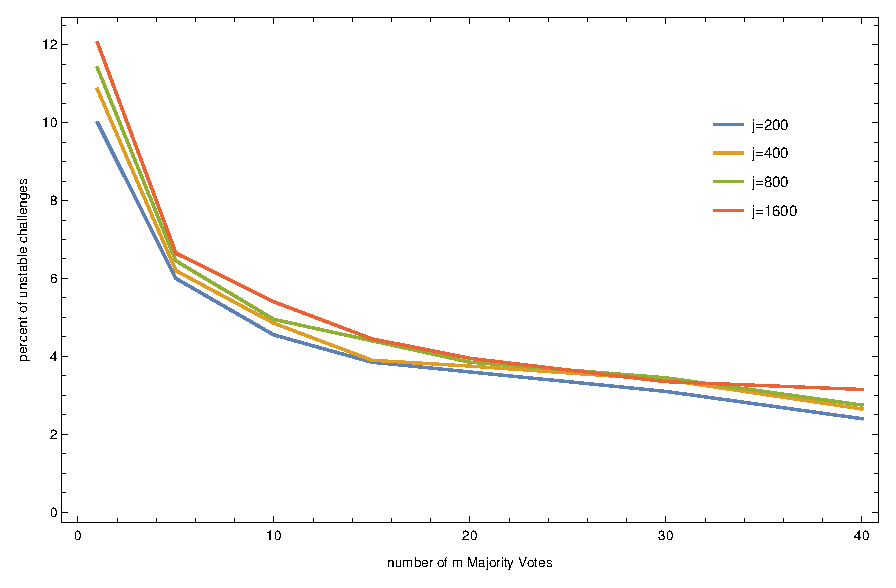
\includegraphics[width=1.00\textwidth]{images/mv-measurements-unstableChallenges.eps}
% \noindent\includegraphics[width=1.00\textwidth, height=3cm, draft]{example-image-a}
\caption{}
\label{fig:cmamajorityvotemeasurementrelation}
\end{figure}

\section{\apufs vs. \mpufs}
% ES-CMA: arbiter vs. mv arbiter
%========================================

\section{\acs{XOR} \apufs vs. Majority \acs{XOR} \apufs}
% ES-CMA: XOR arbiter vs. MV XOR arbiter
%========================================

